\documentclass[10pt,a4paper,twoside]{article}
% The following LaTeX packages must be installed on your machine: amsmath, authblk, bm, booktabs, caption, dcolumn, fancyhdr, geometry, graphicx, hyperref, latexsym, natbib

% Please make sure that spp.dat (supplied with this template) is in your working directory or path
\input{spp2024.dat}

\renewcommand{\P}[1]{\left( #1 \right)}
\renewcommand{\l}{\ell}
\renewcommand{\ref}[1]{Fig. #1}

%  Editorial staff will uncomment the next line
% \providecommand{\artnum}[0]{XX-XX}
% \renewcommand{\articlenum}[0]{SPP-\the\year-\artnum-}

\begin{document}

\title{\TitleFont Gaussian component of beams with fractional topological charge}

\author[*]{Maria Isabella M.~Mendoza~\authorsep}
\author[ ]{Nathaniel Hermosa \authorsep}
\author[ ]{Ni\~na Zambale Simon~\lastauthorsep}
\affil[ ]{National Institute of Physics, University of the Philippines Diliman, Philippines}
\affil[*]{\corremail{mmmendoza31@up.edu.ph} }

\begin{abstract}
\noindent
% [ver. 1 - w/ Ate Ninya's comments]\\
% Laguerre-Gauss (LG) beams of fractional topological charge $l$ are modeled as a superposition of integer-$l$ modes. Fractional vortex beams are interesting (motivation stuff). Offers finer adjustment etc. In this paper, we distinguish LG beams of fractional $l$ by projecting them onto a Gaussian mode. We generate beams with fractional $l$ and passed them into a single mode fiber,  reading the intensity of the exiting beam as voltage. We observe that this voltage is maximum for the Gaussian mode, dropping for succeeding modes but lowest at integer or near-integer $l$ as predicted by orthogonality principles. Moreover, it is nonzero in intermediate values in $l > 1$, especially at $l<2$ [why?]. 
% [ver. 2]\\
% Fractional vortex beams are interesting for allowing finer control of orbital angular momentum (OAM). In this paper, we characterize LG beams of fractional $l$ by projecting them onto a Gaussian mode. We generated beams with fractional $l$ using an SLM and passed them into a single mode fiber, recording the magnitude of the output (projection) as voltage. We observe that this voltage is maximum for the Gaussian mode, dropping for succeeding modes but lowest at integer or near-integer \$l\$ as predicted. Moreover, we observe that the Gaussian component still manifests at fractional $l$. We think this is due to the absence of vortices on the z-axis as stated by Berry; it peaks at half-integer $l$ because [state reason here], but diminishes overall with increasing $l$ due to [reason]. [Put conclusion].
% [ver. 3]
Fractional vortex beams, which possess fractional topological charge $l$, are interesting for allowing finer control of orbital angular momentum (OAM). In this paper, we characterize these kinds of beams by projecting them onto a Gaussian mode. We generated beams with fractional $l$ using an SLM and passed them into a single mode fiber, recording the magnitude of the exiting beam as voltage. We observe that this voltage is maximum for a Gaussian beam ($l=0$) and lowest at or near integer $l$ as predicted. Moreover, we observe that the Gaussian component still manifests at fractional $l$; we believe this is due to the absence of vortices on the z-axis as described by Berry~\cite{Berry}. Our results have provided an alternative method to describe fractional vortex beams, as well as empirical validation for Berry's theoretical work on the fractional vortex beam.

%Specifically, it peaks at half-integer $l$ because [state reason here], but diminishes overall with increasing $l$ due to [reason]. 

\keywords{vortex beams, fractional topological charge, single-mode fiber, mode projection}

\end{abstract}

\maketitle
\thispagestyle{titlestyle}


%--------------------------------------------------
% the main text of your paper begins here
%--------------------------------------------------

\section{Introduction}\label{sec:intro}
% Vortex beams have been used in fields such as information encoding and particle manipulation, for their orbital angular momentum (OAM) \cite{rev-trap}. 

% As solutions to the free-space Helmholtz equation in cylindrical coordinates, their fields exhibit radial symmetry \cite{rev}: 
% Directly related to the OAM of vortex beams \cite{alperin} is their azimuthally-varying phase $i\l \phi$, or a helical wavefront. Indeed, this phase manifests as a dark central region --- a vortex --- resulting from the spiraling paths of photons about the propagation axis \cite{twisted}.
% The OAM manifests as a dark central region, which results from an azimuthally-varying phase $\P{il\phi}$ in the equation of the field (in cylindrical coordinates)\cite{twisted, rev}:

%In particular, $l$, the topological charge, signifies the number of "turns" made in one circular scan of the transverse profile; integer values of $l$ manifest as a larger central region. %The OAM of a vortex beam is directly proportional to $l\hbar$. Describe this as (related to) the eigenvalue of the free space Helmholtz equation

% The modes of vortex beams, arising from the free-space Helmholtz equation, are differentiated by the values of $l$; as the eigenmodes, integer modes are the most readily used for the applications of OAM mentioned above. 

% are you focusing on modal decomposition or mode projection????
% Modal decomposition of a beam into a complete basis set can be done through projection of the beam on diffractive elements (e.g. SLM, spiral phase plate, or an optical fiber).

% ----
Vortex beams are an example of beams carrying orbital angular momentum (OAM), which manifests as a central region of zero intensity --- a vortex. As such, they have been leveraged in fields like particle manipulation, information encoding, and imaging \cite{rev-trap}. 
% they (their fields) are radially symmetric
Their OAM results in a helical wavefront according to their equation of field \cite{rev}:
\begin{align}
    \psi(r,\phi, z) \propto \exp\P{-\frac{r^2}{w_o^2}} \exp(i\ell\phi)
\end{align}
and is directly proportional to the "twists" of this wavefront given by the topological charge $\ell$ \cite{alperin, twisted}.
% a helical wavefront, or an azimuthally-varying phase $i\l \phi$.
% Indeed, this phase manifests as a dark central region --- a vortex --- resulting from the spiraling paths of photons about the propagation axis \cite{twisted}.
%In particular, $l$, the topological charge, signifies the number of "turns" made in one circular scan of the transverse profile
%The OAM of a vortex beam is directly proportional to $l\hbar$. Describe this as (related to) the eigenvalue of the free space Helmholtz equation
% the 'topological charge' of the beam, which signifies the number of "turns" made in one circular scan of the transverse profile
The modes of vortex beams $\psi_\ell$ are differentiated by the values of $\ell$. As the eigenmodes, integer modes are the most readily used for the applications of OAM mentioned above. However, the interest in fractional modes has been growing in recent years, with their intermediate OAM values enabling finer control in the applications mentioned above \cite{rev}.

The structure of fractional modes has been predicted by Berry to be a chain of off-axis vortices, arising from their expression as a superposition of integer modes \cite{Berry}. The field of a paraxial fractional mode is given in cylindrical coordinates by:
 \begin{align}
  \psi_\ell (R, \phi, z) &= \frac{\exp\P{i\pi \ell} \sin\P{\pi \ell}}{\pi}
  \sum_{n=-\infty}^{\infty} \frac{1}{\ell - n} \psi_n (R, \phi, z)
\end{align}\label{eq:parax}

\noindent where $R$ is the position --- and $\phi$ the azimuthal angle --- on a perpendicular plane to the propagation axis $z$, $n$ is an integer, and $\ell$ is a fraction.

The arrangement of these integer vortices in a fractional vortex beam has also been shown experimentally in terms of both intensity and phase \cite{exp-struc, fiber-struc}. However, also predicted by Berry is the absence of vortices on the z-axis \cite{Berry} --- that is, the phase no longer has azimuthal dependence at $R=0$:
\begin{align}
     \psi_\ell (R=0, z) &= \frac{\exp\P{i(z + \pi \ell)} \sin\P{\pi \ell}}{\pi \ell}
\end{align}\label{eq:vortz}

In this work, we experimentally generate fractional vortex beams, and investigate their resulting intensity and mode. We measure the Gaussian component of these beams by projecting them on a Gaussian mode provided by a single mode fiber. In contrast to the mentioned experiments, whose focus is on the arrangement and stability of these vortices, we aim to describe these vortex beams instead by the absence of vortices on the z-axis. This is equivalent to examining their Gaussian ($\ell=0$) component, which can be done through a Gaussian single mode fiber.

% is there another advantage (ex. resolution) of analyzing the results of an optical fiber rather than direct images?

\section{Methods}\label{sec:methods}
% path of the laser?
Figure \ref{fig:setup} shows the schematic diagram of the experimental setup used to generate and characterize fractional vortex beams. A beam from a He-Ne laser ($\lambda= 633$ nm) is expanded using a set of lenses and illuminated the surface of a spatial light modulator (SLM -- Pluto Holoeye). We uploaded holograms $H$ onto the SLM of the fractional vortex beams of the form,

\begin{equation}
    H \propto {|E_{obj} + E_{ref}|}^2 
\end{equation}

\noindent where $E_{obj}$ is the electric field of the fractional vortex given in equation \eqref{eq:parax}, and $E_{ref}$ is the electric field of the reference beam. Upon reflecting off from the SLM, we isolated the first diffractive order using a pinhole. The intensity profiles of these fractional modes were captured using a CCD camera (Point Grey FlyCap). 

% Gaussian mode projection
Next, to measure the strength of the Gaussian mode, we use a single mode fiber (SMF) connected to a photodetector that measures the intensity as voltage. This photodetector is connected to the oscilloscope for us to record the optical signal. We removed the beam splitter in the experimental setup to allow the full intensity into the SMF. The beam size is further reduced by a pair of lenses for it to fully fit into the fiber. The exiting beam --- the projection -- is registered in the photodetector and the corresponding voltages were measured by the oscilloscope at 2500 samples/second. We vary the value of $\l$ from 0.0 $\le \l \le 5.0$ with interval of 0.05. 

% $1$ was varied at 0.05 interval for $l \in [0, 1.0]$, then at 0.1 interval until $l=5.0$. 

% 
%These voltages were recorded to a USB for $0.0 \le l \le 5.0$.% $1$ was varied at 0.05 interval for $l \in [0, 1.0]$, then at 0.1 interval until $l=5.0$. 
%They were then corrected for background signal and the photodetector gain (40 dB). The voltage and uncertainty for each $l$ were represented as the mean and standard error, respectively, then plotted in \cref{fig:V}.

%Beams of different fractional $l$ were generated by a spatial light modulator (SLM), to capture images of their transverse intensity profiles and to propagate them through a Gaussian single mode fiber (SMF).
% how l is varied
%$l$ is set by a MATLAB script, which uploads to the SLM a hologram (an 8-bit grayscale image) that represents the phase change in the spatial profile of the beam.

\begin{figure}[h!]
    \centering
    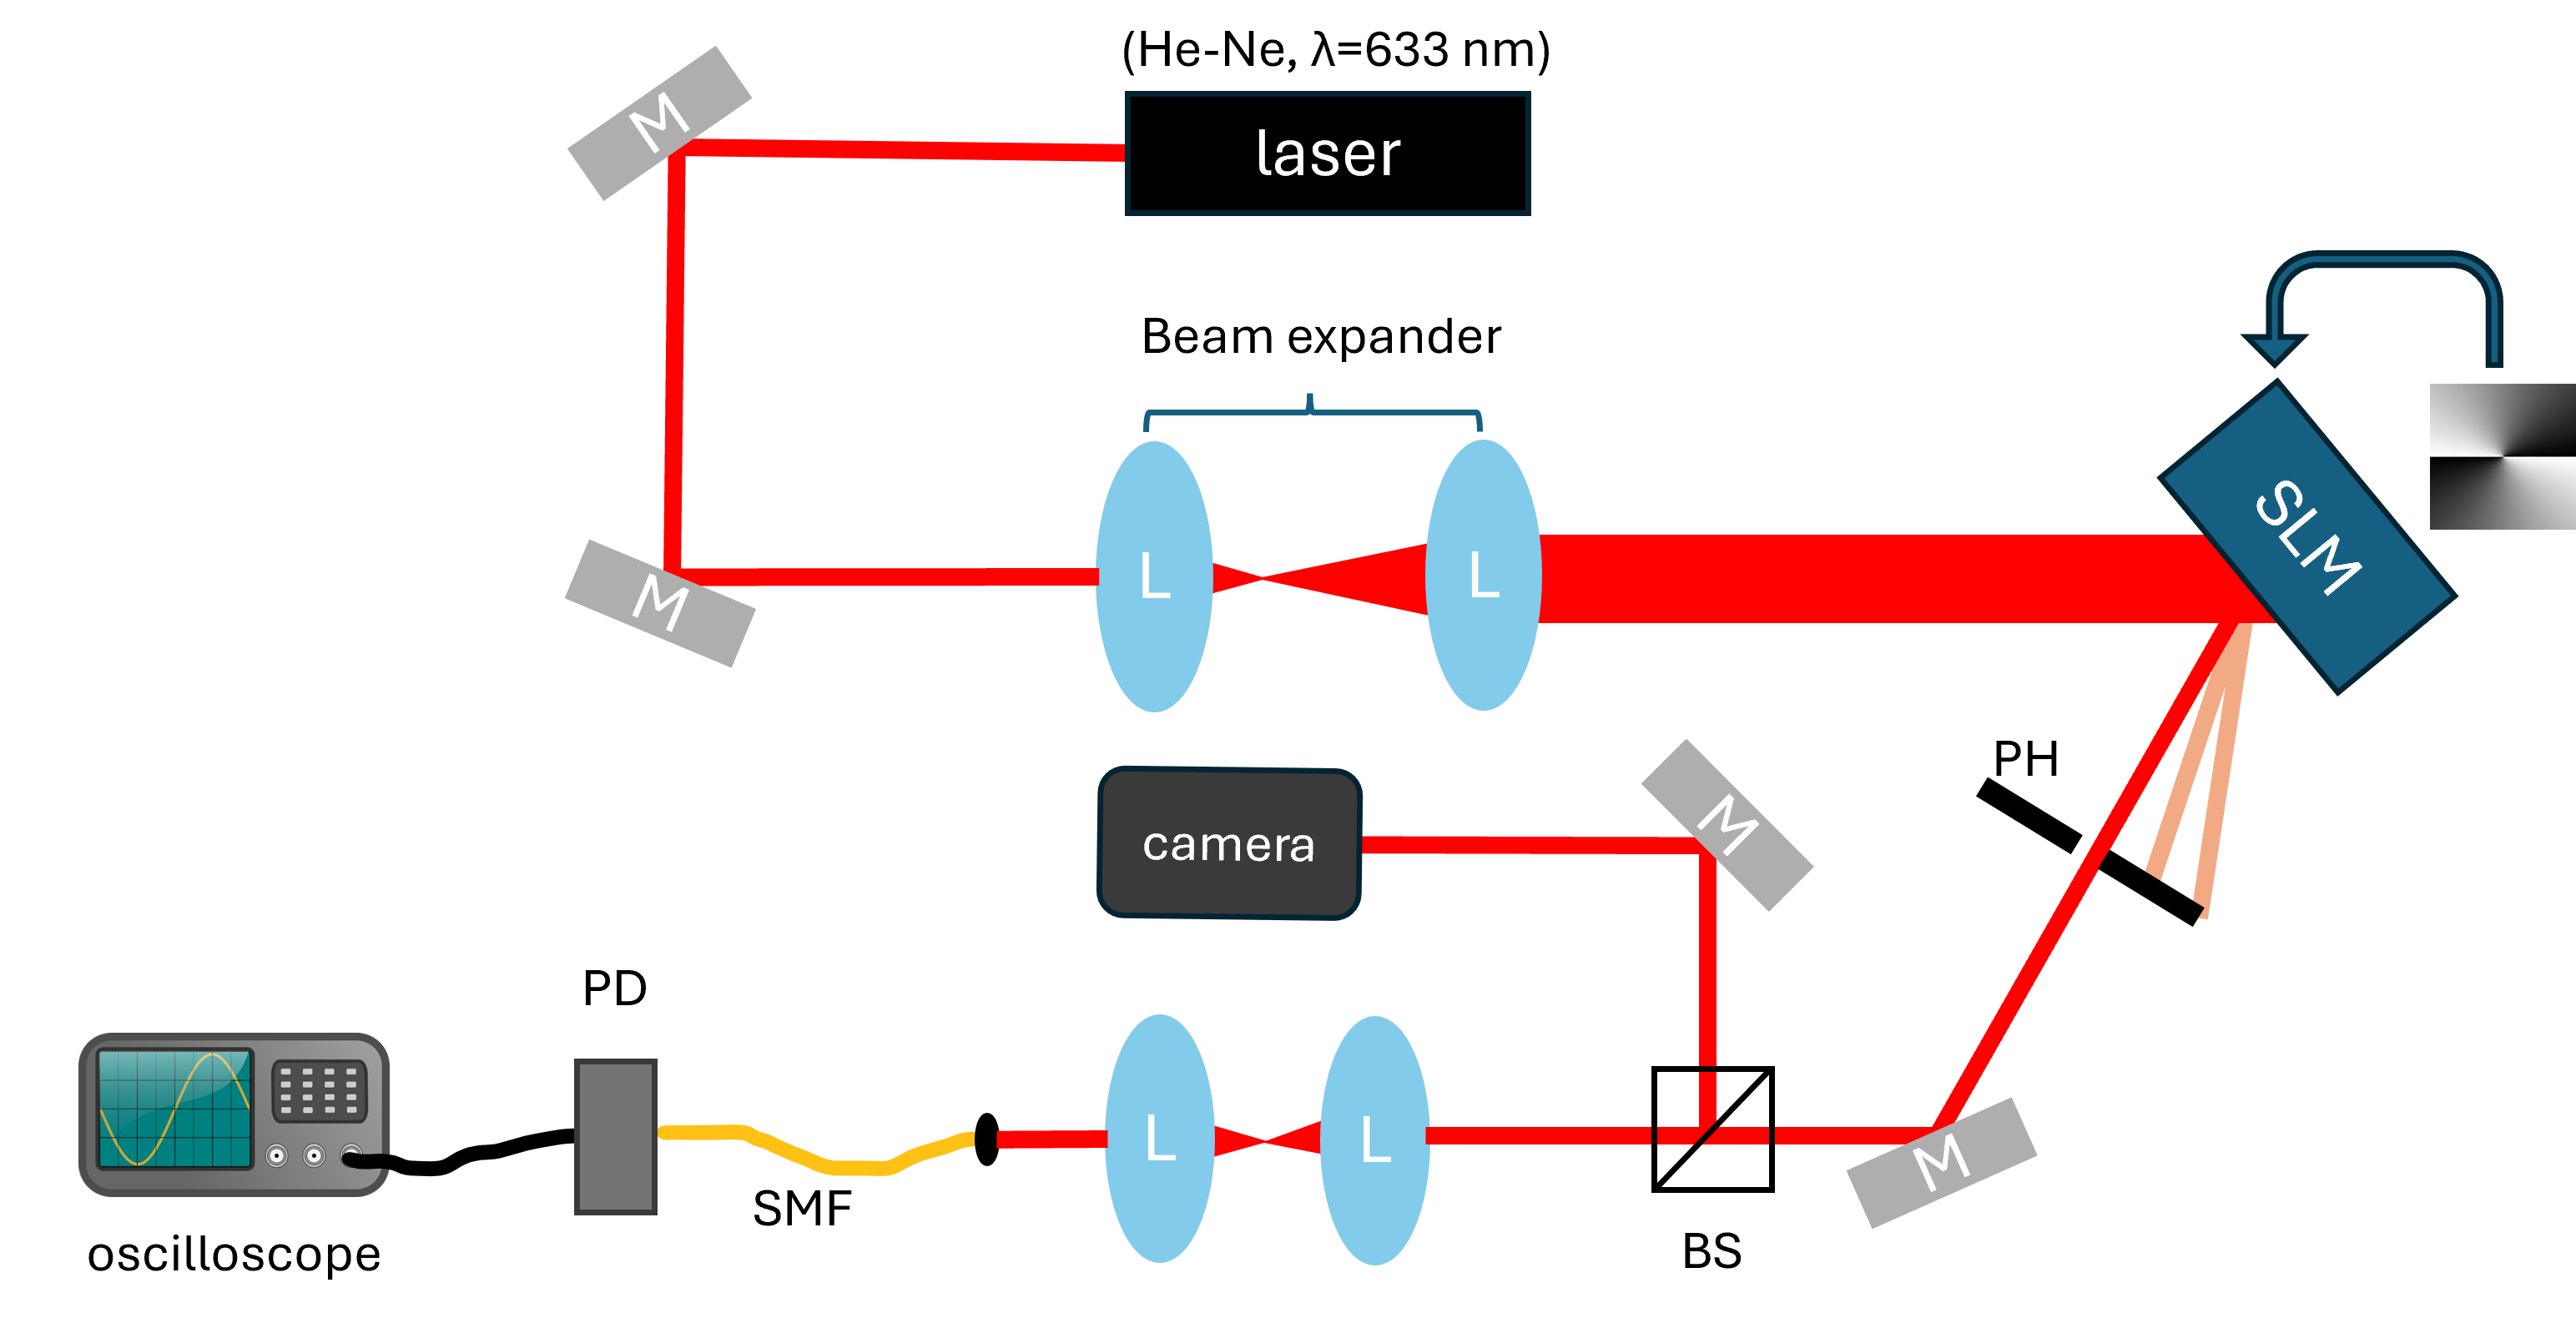
\includegraphics[width=0.7\textwidth]{setup.png}
    \caption{Schematic diagram of the experimental setup. Collimated light from the laser hits the surface of the SLM where the hologram of the fractional vortex beam is uploaded. We select the first diffraction order using a pinhole (PH) and mirror (M),  measure the corresponding Gaussian component using a single mode fiber (SMF) connected to a photodetector (PD) as we change the value of $\l$. } 
    %Isingit dapat sa caption yung mga acronyms. 
    %\\(He-Ne = helium-neon (gas) laser; M = mirror; L = lens; SLM = spatial light modulator; PH = pinhole; BS = beam splitter; SMF = single mode fiber; PD = photodetector)}
    \label{fig:setup}
\end{figure}

\section{Results \& Discussion}\label{sec:rnd}

\begin{figure}[h!]
    \centering
    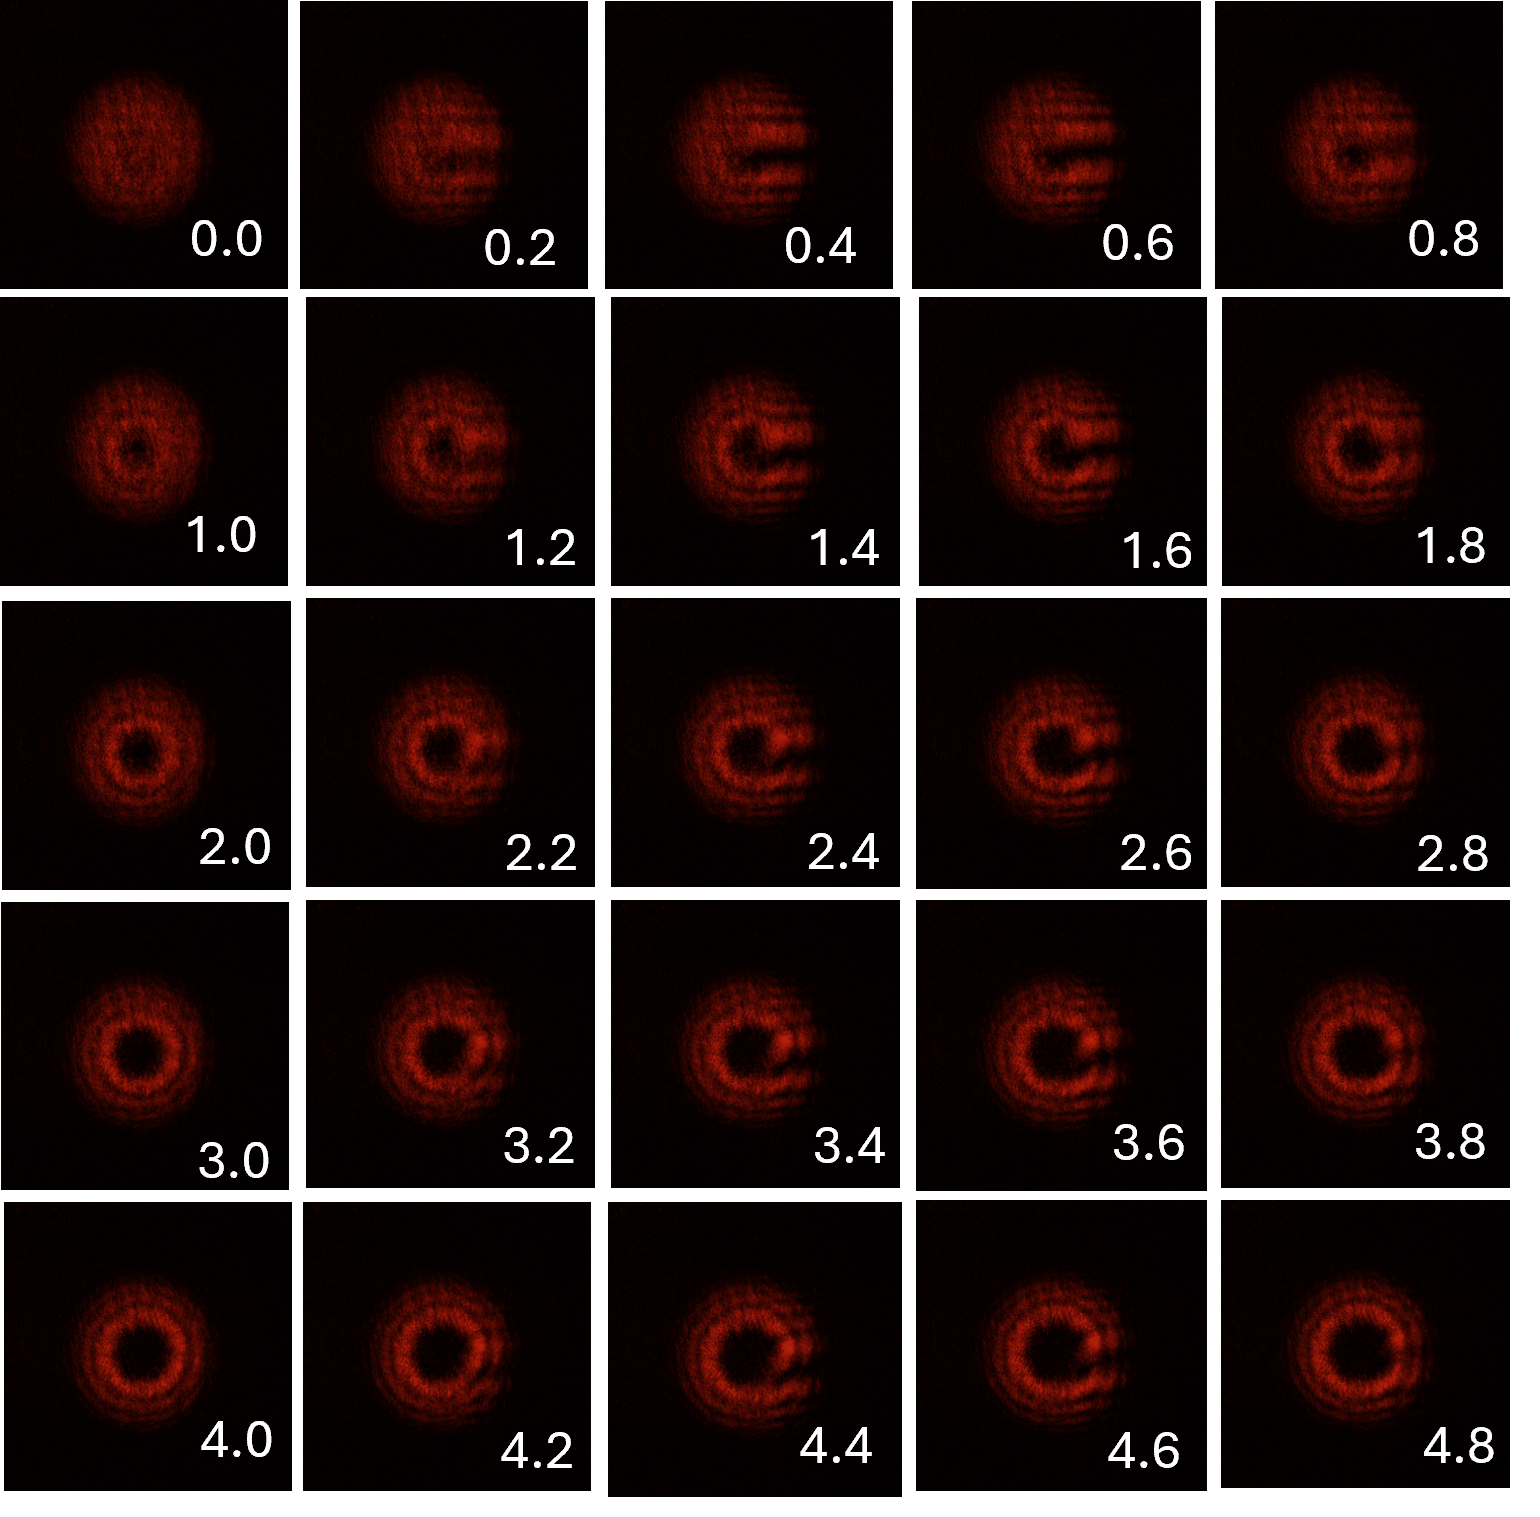
\includegraphics[width=0.5\textwidth]{intensities.png}
    \caption{Intensity profiles of vortex beams at different $0.0 \le \ell \le 5.0$. Non-integer vortex modes have a characteristic ``tear" on their right side, unlike the uniform distribution of Gaussian mode ($\ell = 0$) and doughnut modes (integer $\ell$.) }
    \label{fig:I}
\end{figure}

% Comments on intensity profiles
One of the distinguishing features of integer vortex beams is the dark region at their center, resulting from the phase singularity. This characteristic is why these beams are also referred to as doughnut modes. Figure \ref{fig:I} shows the experimentally generated fractional and vortex beams with the setup shown in Figure \ref{fig:setup}. Among integer vortices, we observe that a larger $\l$ corresponds to a larger dark central region, consistent with previous results~\cite{padgett2015divergence}. However, when having non-integer or fractional topological charges, dark stripes and circular fringes arise as seen in the figure. These features exhibit the evolution of the vortex wherein it begins from a ``tear" on the right side and then gets absorbed by the dark region forming larger vortices. Also noticeable on profiles of $\l \ne 0$ are dark concentric rings. These features can be attributed to the edge-diffracted waves described by the Bessel function in \eqref{eq:parax}, formed when we use fractional topological charges $\l$ as calculated by ~\cite{Berry}. 

\begin{figure}[h!]
\centering
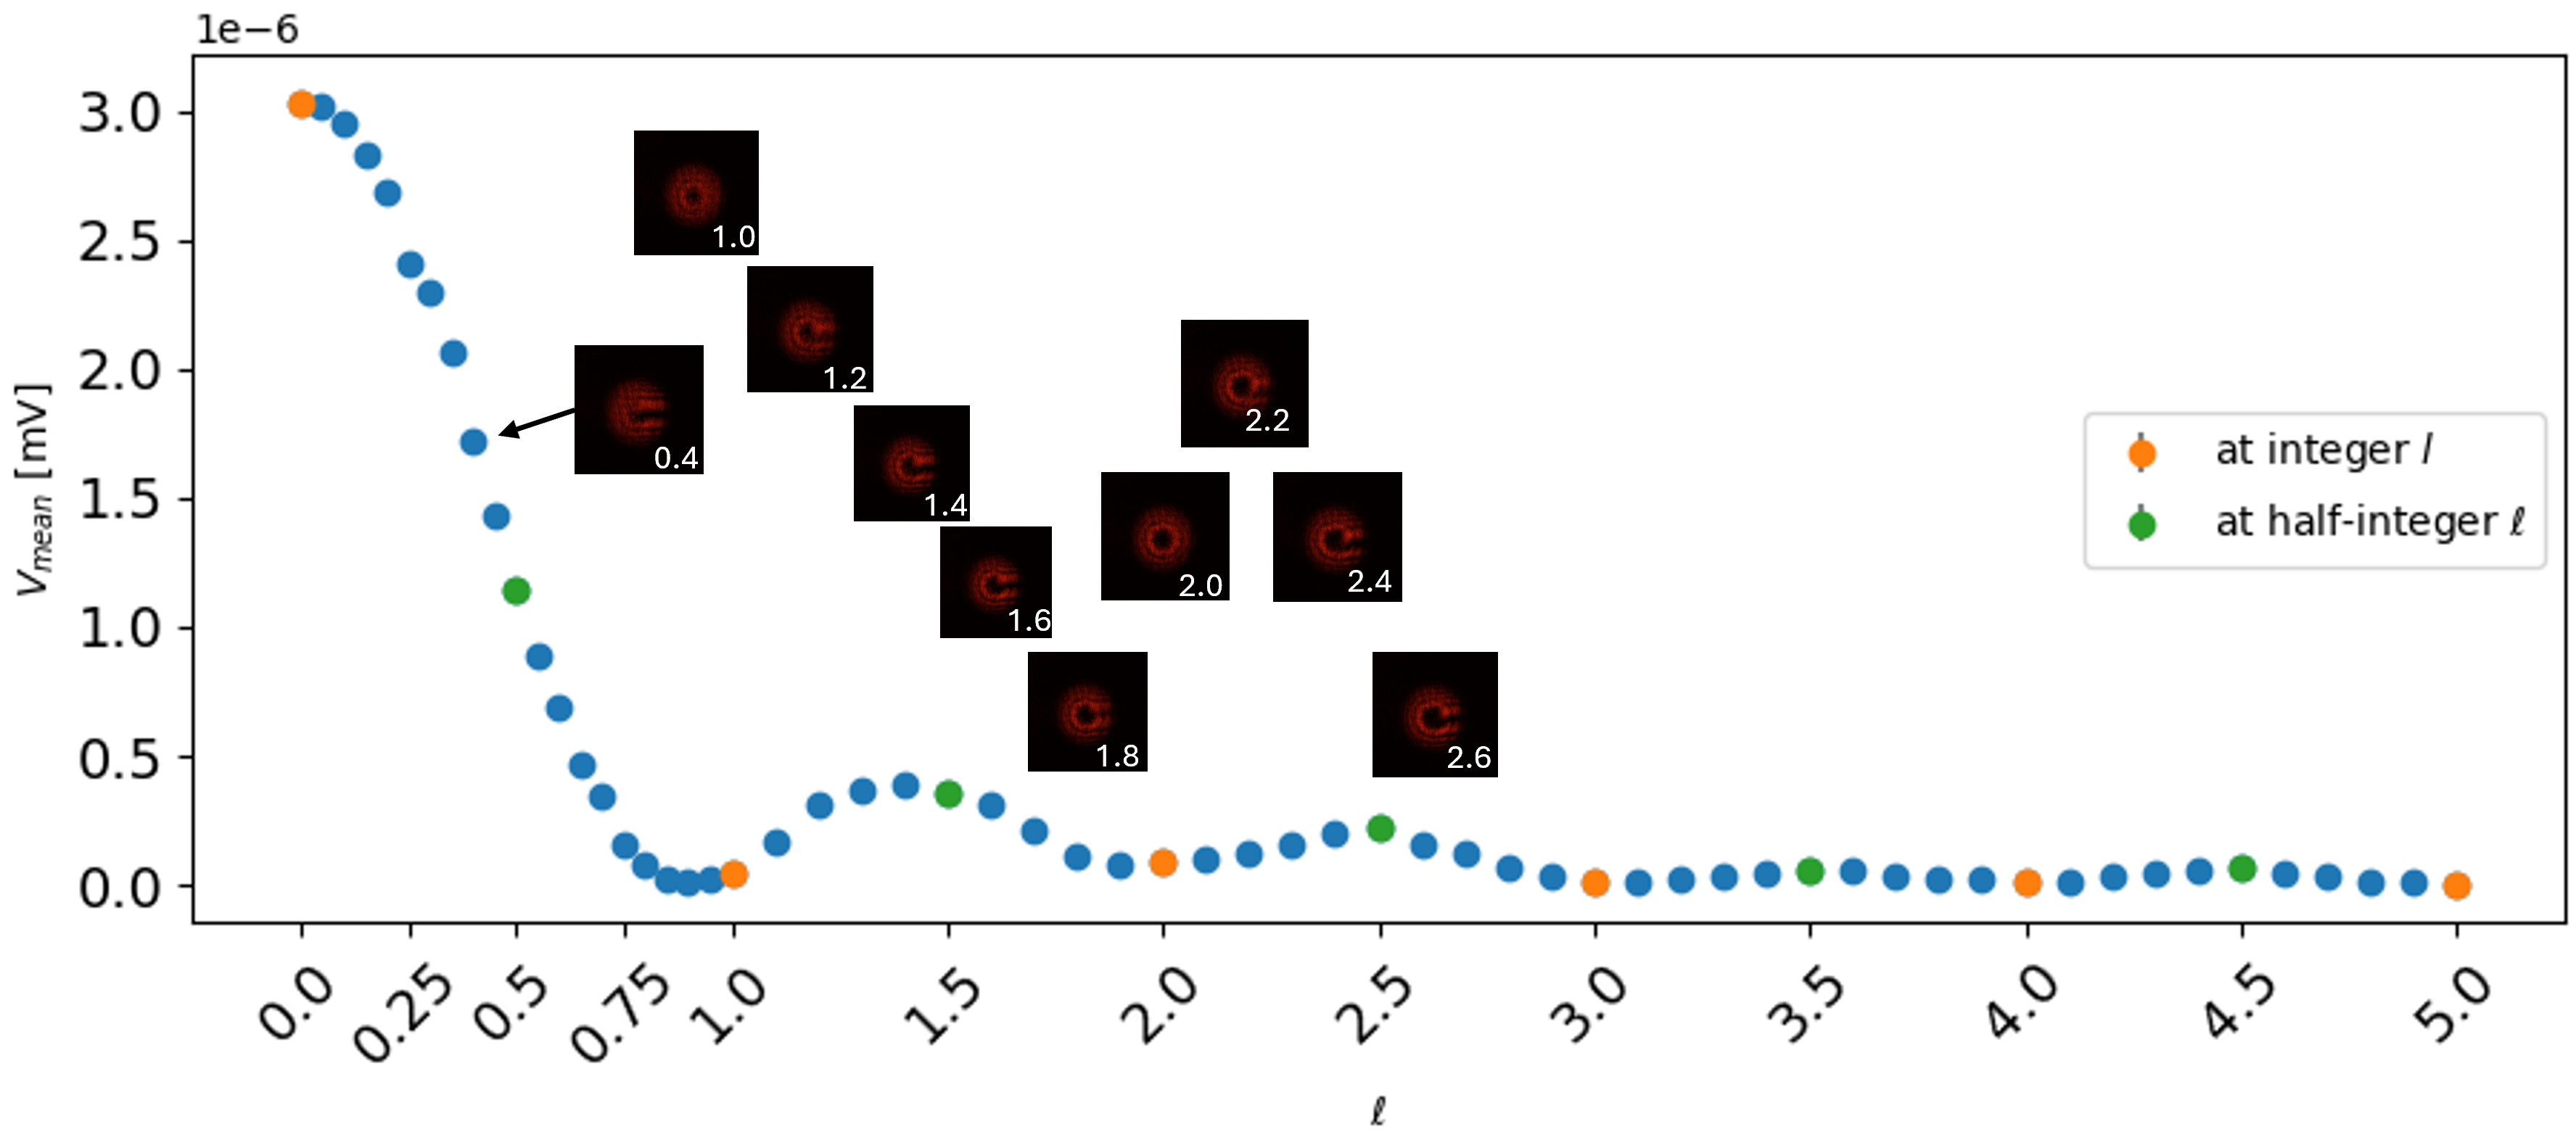
\includegraphics[width=0.85\textwidth]{SMF.png}
\caption{Mean voltage $V_{mean}$ representing the Gaussian component at each value of $\ell$. The errorbars (gray) are obscured by the markers. The voltage curve has local peaks for half integer values of $\ell$ (e.g. $\ell = 1.5, 2.5$).}
\label{fig:V}
\end{figure}

% Comments on the Gaussian component
From the raw voltage reading from the oscilloscope, we obtain mean voltage reading per fractional charge $\ell$ to get the Gaussian component of the fractional vortex as shown in Figure \ref{fig:V}. As expected, the curve peaks at $\ell = 0$ where the incident beam coincides with the mode of the single mode fiber. We also observe that for integer values of $\ell \neq 0$, the voltage is close to zero which can be explained by orthogonality principles between the incident light and the mode of the SMF. % recall, the mode of the single mode fiber is a Gaussian ($\l=0$)

However, a different phenomenon occurs when the topological charge is fractional, especially when $\ell$ is near half-integer values. Looking at just the images, it is not immediately intuitive that the Gaussian component would peak at half-integers for $\ell > 1$. But, as seen in the voltage curve, we observe peaks near half-integer values (e.g., $\ell = 1.5, 2.5$, etc.). We believe these peaks arise due to the occurrence of $\ell = 0$ modes. As first predicted by Berry~\cite{Berry} and experimentally demonstrated by Leach et al. using phase measurement techniques~\cite{leach2004observation}, for half-integer $\ell$ values, a line of alternating charge vortices forms near the radial discontinuity. These alternating charge vortices result from the birth of a vortex that occurs when $\ell$ passes a half-integer step. Since the nearest integer to the fractional vortex $\ell$ increases by unity when $\ell$ passes a half-integer step, an extra vortex must be created~\cite{Berry}. Additionally, we observe an overall decrease in the peaks as $\ell$ increases, which may be explained by the increasing radius of the central dark region, as seen in the images of the integer modes in Figure \ref{fig:I}.

%These peaks arise due to the total vortex strength, which is step-wise, increases at half-integer values $\ell$~\cite{Berry}. However, another thing to consider is the specific arrangement of the vortices at these half-integers. In particular, half-integer vortices are comprised of a chain of same-$\ell$ vortices of alternating sign. 

%More specifically, Berry also models the so-called "total vortex strength", which increases with $\l$ (you may quote the figure from Berry???). This strength, which is step-wise, increases at half-integer values; 

%Moreover, the deviation of $\l$ from integer values exhibits a Gaussian mode that increases gently. This too is consistent with another of Berry's predictions --- that the vortices will be near the z-axis.

%These indicate that the dark region for fractional modes has only low but non-zero intensity 

%--- a feature anticipated as well in \cite{Berry}. 

%The observed dip in the strength of the Gaussian at integer or near-integer $l > 0$ is consistent with the orthogonality of the integer modes.

%[And so???] In contrast to non-half-integer values... what do those look like? what do you mean by "annihilation" of the chain away from half-integer values and how does that impact the appearance of the projection through the SMF?

%[Explain, on the other hand, if there's time, why the Gaussian weakens monotonously at fractional values of $l \in [0.0, ~1.0]$.]

% comment --- find sources --- on the specific arrangement of the vortices around the z-axis. Then relate it to the weakening Gaussian component at higher l

% Recommendations


\section{Conclusions}
% What is the significance of our findings?
% \begin{itemize}
%     \item Simulates some kind of turbulence?
%     \item Vice versa from our results - for deliberately generating fractional topological charge
%     \item Then this permits various applications - as an alternate method to generate fractional OAM; to gain information about the environment where light propagates in, etc.
% \end{itemize}

In this study we have projected fractional vortex beams onto a Gaussian mode carried by a single mode fiber to study their Gaussian component. We analyzed our results, guided both by the predictions of Berry --- as well as the intensity profiles which were consistent with these predictions. In particular, we focused on the Gaussian components at (and near) integer and half-integer $\l$, showing consistency with Berry's predictions as well. Our results have thus demonstrated the study of the Gaussian component --- or the absence of vortices --- as an alternate description of fractional vortex beams, without looking at the precise positions of the vortices in the beams themselves.

Although we have attributed the qualities of our images and Gaussian component to the predictions of Berry, we recommend to calculate the specific power of the mode projection between the fractional vortex and the Gaussian mode to get a more precise description of the Gaussian component of the beam. This can be done by evaluating the overlap integral $\int \psi_{\l}^* \psi_{0}~dA$ over cross-sectional area $dA$ where $\psi_0$ is the Gaussian mode of the single mode fiber. To verify the existence of other modes in fractional vortex beams, one can also implement a modal decomposition similar to \cite{vasnetsov2005analysis}. Additionally, our methods may be extended, as an alternate characterization, to previous studies \cite{fiber-struc} of the fractional vortices at different propagation distances.

%\begin{equation}
    % \text{setup the integral}
 %   \int \psi_{\l}^* \psi_{\l=0} dA
%\end{equation}
%which is over the cross-section differential $dA$.



\section*{Acknowledgments}
The authors would like to thank DOST hilippine Council for Industry, Energy and Emerging Technology Research and Development (PCIEERD Project No. 04002),and the 
University of the Philippines Office of the Vice President for Academic Affairs thru its Balik-PhD Program (OVPAA-BPhD 2015-06) for financial support. NZ Simon would like to acknowledge the Office of the Chancellor of the University of the Philippines Diliman, through the Office of the Vice Chancellor for Research and Development, for funding support through the Thesis and Dissertation Grant (Project No. 232310 DNSE).

% \section*{*Additional Reminders}
% \begin{itemize}
%     \item The most common cause of manuscript processing delays is incorrect formatting of the (1) author block and affiliation bylines, and (2) references. Please verify that all blue web hyperlinks resolve correctly.
%     \item The Full Proceedings is also prepared in print. Please follow the maximum page limit of Four (4) pages \textit{including references}. 
% \end{itemize}

% Please use the style file spp-bst.bst. If you wish to use BibTeX, kindly use us the filename bibfile.bib for your bib file.
\bibliographystyle{spp-bst}
\bibliography{bibfile}

\section*{Appendix}

This Github repository (https://github.com/mimmphi/phase-holes-SPP-MIMM) contains the MATLAB program (SLM control), Python program (data processing), and raw data.

\end{document}